\chapter{الگوریتم‌های کوانتومی‌}
در حال حاضر، چندین الگوریتم کوانتومی وجود دارد. این الگوریتم‌ها، کیوبیت‌ها را به صورتی تغییر میدهند که مسائل را حل کنند. به طور کلی، این الگوریتم‌ها کارایی بالاتری از الگوریتم‌های کلاسیک معادل خود دارند و باید هم چنین باشد زیرا در غیر این صورت، استفاده از کامپیوترهای کلاسیک و الگوریتم‌های کلاسیک، گزینه بهتری خواهد بود. 
\\
همه الگوریتم‌های کوانتومی 4 مرحله ی یکسان را دنبال میکنند:
\begin{enumerate}
\item
هنگام شروع به کار سیستم، کیوبیت‌ها در یک حالت کلاسیک خاص قرار دارند(صفر یا یک)
\item
سیستم در حالت برهم‌نهی میرود
\item
سپس با اعمال گیت‌ها و عملیات مختلف، احتمالات برهم‌نهی تغییر پیدا میکند
\item
در نهایت، کیوبیت ها اندازه‌گیری میشوند
\cite{cambridgebook}
\end{enumerate}
در الگوریتم‌های کوانتومی، از آنجایی که کیوبیت‌ها و حالات دارای احتمال هستند، همیشه با ورودی‌های یکسان، خروجی یکسان نخواهد بود. با انجام یک الگوریتم بر روی یک ورودی مشخص بارها و بارها، میتوان احتمال هر خروجی را بدست آورد. معمولا، جواب درست، از لحاظ احتمالاتی، فاصله زیادی با دیگر خروجی‌ها دارد.
\section{الگوریتم دویچ}
الگوریتم دویچ
\LTRfootnote{Deutsch's algorithm}
ساده‌ترین الگوریتم کوانتومی است. فرض کنید تابعی داریم به نام $f$ که فضای ورودی آن $\{0, 1\}$ و فضای خروجی آن $\{0, 1\}$ است. در این تابع، اگر $f(0) != f(1)$ باشد، تابع متعادل است و اگر $f(0) = f(1)$ باشد، تابع ثابت است.
فرض کنید نمیدانیم تابع از کدام نوع است و میخواهیم نوع تابع را مشخص کنیم. در الگوریتم کلاسیک، برای بدست آوردن جواب، دو بار فراخوانی تابع نیاز است. اما با استفاده از الگوریتم دویچ و محاسبات کوانتومی، با یک بار فراخوانی تابع به جواب میرسیم. ابتدا مسئله را مدل میکنیم.
\ref{eq:deutsch}
\begin{equation} \label{eq:deutsch}
f(x)  \oplus f(y) = \left\{ \begin{array}{cl}
1 & : \ \verb; f is balanced; \\
0 & : \ \verb; f is constant;
\end{array} \right.
\end{equation}
تابع کوانتومی معادل با $f$ را میتوان با یک ماتریس نشان داد. این تابع برگشت‌پذیر است و دو کیوبیت دریافت میکند و حاصل آن نیز دو کیوبیت با احتمالا متفاوت است. در نمایش ماتریسی، ردیف بالا خروجی ها و ستون چپ، ورودی ها را نشان میدهد.
\ref{fig:deutschunitery}
\ref{fig:deutschmatrix}
\begin{figure}[!h]
\centerline{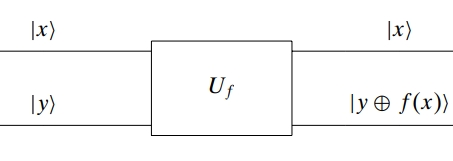
\includegraphics[width=.5\textwidth]{deutschunitery.jpeg}}
\caption{تابع کوانتومی ارزیابی $f$}
\label{fig:deutschunitery}
\end{figure}

\begin{figure}[!h]
\centerline{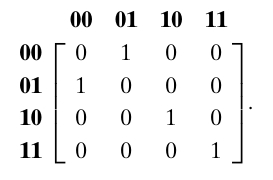
\includegraphics[width=.4\textwidth]{deutschmatrix.jpeg}}
\caption{بازنمایی ماتریسی تابع کوانتومی ارزیابی $f$}
\label{fig:deutschmatrix}
\end{figure}
حال، باید مداری طراحی کنیم که ابتدا دو کیوبیت جامد(در حالت ساده فیزیک) را به حالت برهم‌نهی ببرد، تابع ارزیابی را روی آنها اعمال کند و درنهایت، با تبدیل دوباره کیوبیت‌ها به حالت جامد، آنها را اندازه‌گیری کند. دویچ، مدار شکل
\ref{fig:deutschcircuit}
 را درنظر میگیرد.
\LTRfootnote{solid-state qubit}
\begin{figure}[!h]
\centerline{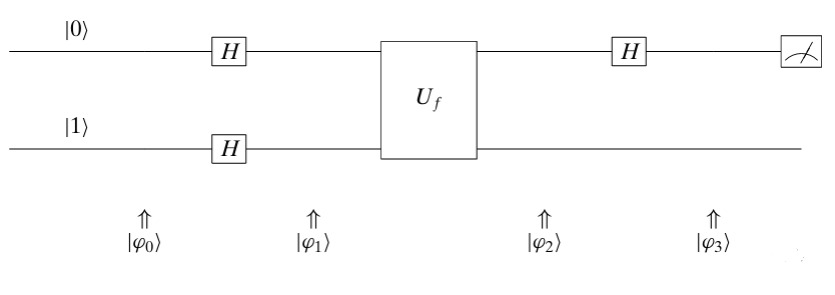
\includegraphics[width=.8\textwidth]{deutschcircuit.jpeg}}
\caption{مدار نهایی الگوریتم دویچ}
\label{fig:deutschcircuit}
\end{figure}
برای راحتی دنبال کردن چرایی کارایی این الگوریتم و آشنایی با معادلات کوانتومی، حالت کیوبیت‌ها در هر مرحله زمانی از الگوریتم به نمایش گذاشته‌شده است.
\ref{fig:deutschproof}

\begin{enumerate}\addtocounter{enumi}{-1}
\item
ورودی بالا را کیوبیت جامد با مقدار صفر و ورودی پایین را با مقدار یک قرار میدهیم.
\item
با اعمال گیت هادامار
\LTRfootnote{Hadamar's gate}
،
کیوبیت ها را به حالت برهم‌نهی میبریم. 
\item
در اینجا، مقدار های نامشخص $f$ را در معادله قرار میدهیم. درنهایت، جواب بدست آمده، این مقادیر را مشخص میکنند. در نتیجه، با استفاده از خروجی میتوانیم نوع تابع را مشخص کنیم.
\item
تابع هادامار برگشت‌پذیر است و با اعمال دوباره آن، تاثیر اولیه‌اش را از بین میبریم.
\end{enumerate}
\begin{figure}
\centerline{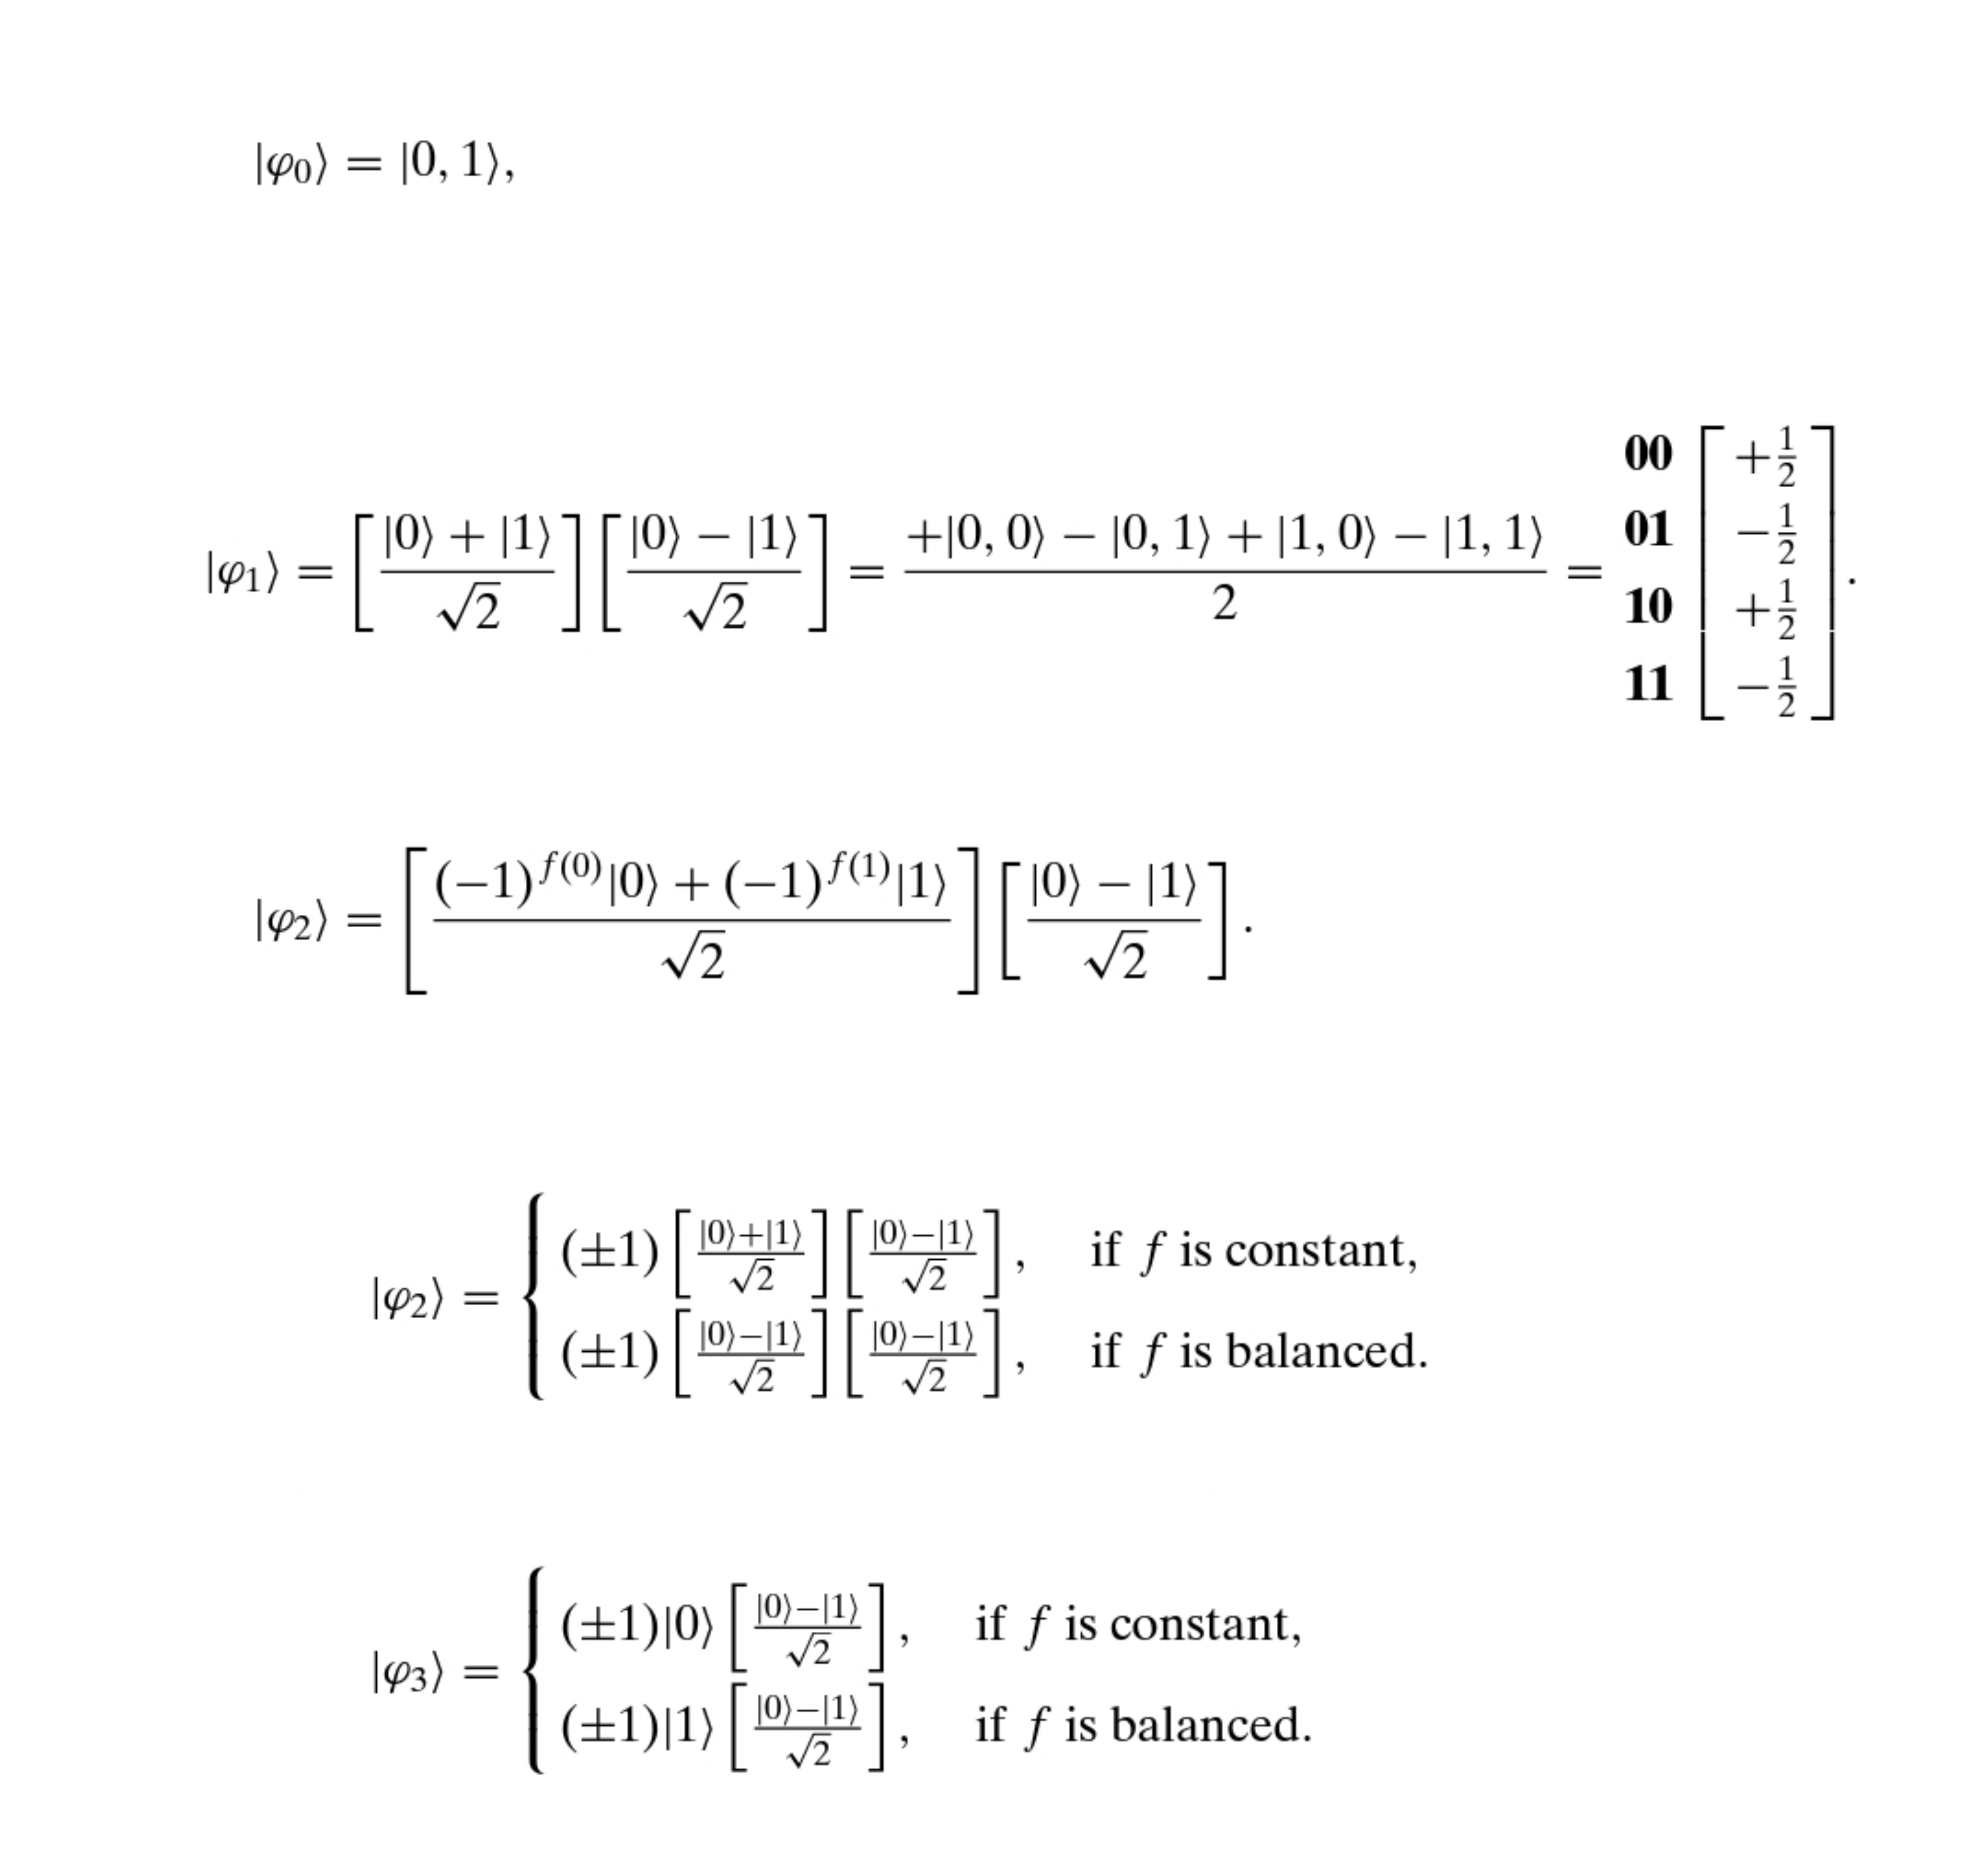
\includegraphics[width=1\textwidth]{deutschproof.jpg}}
\caption{حالت کیوبیت‌ها در هر مرحله از مدار}
\label{fig:deutschproof}
\end{figure}
و در نهایت، کیوبیت بالایی اندازه‌گیری میشود. اگر در حالت صفر قرار داشته باشد، تابع ثابت است و اگر در حالت یک باشد، تابع متعادل است. برتری الگوریتم کوانتومی این است که با یک بار ارزیابی، به جواب مسئله میرسیم که نصف قدم های الگوریتم کلاسیک است. هدف این الگوریتم این است که نشان دهد محاسبات کوانتومی میتوانند از محاسبات کلاسیک کارآمد تر باشند.
\cite{cambridgebook}

\section{الگوریتم گراور}
یکی از مسائل همیشگی کامپیوتر، پیدا کردن یک المان خاص در یک آرایه نامرتب با طول $m$ است. در حالت کلاسیک، برای اینکار در بدترین حالت، $m$ درخواست باید انجام دهیم و در حالت میانگین به $m/2$ درخواست نیاز است. الگوریتم گراور
\LTRfootnote{Grover's algorithm}
این زمان را به $\sqrt{m}$ درخواست تقلیل میدهد. البته چنین کاهش سرعتی در مقایسه با افزایش سرعت نمایی، چندان به چشم نمی‌آید. 
\\
جزئیات ریاضی این الگوریتم طولانی است درنتیجه در این بخش بیان نمیشود. اما کلیاتی از الگوریتم گراور را بیان میکنیم. ابتدا مسئله را مدل میکنیم. $x_{0}$ المان موردنظر است و آرایه هم طول $2^{n}$ دارد.
\ref{eq:grover}
\begin{equation} \label{eq:grover}
f(x) = \left\{ \begin{array}{cl}
1 & : if x = x_{0}  \\
0 & : if x \neq x_{0}
\end{array} \right.
\end{equation}
مراحل الگوریتم گراور برای آرایه با طول $2^{n}$:
\ref{fig:grovercircuit}
\begin{enumerate}
\item
تعداد $n$ کیوبیت با حالت صفر برمیداریم
\item
گیت هادامار $n$ تایی به رویشان اعمال میکنیم و کیوبیت‌ها را به حالت برهم‌نهی میبریم. 
\item
این مراحل را $\sqrt{2^{n}}$ بار تکرار میکنیم

\begin{enumerate}
\item
عملیات معکوس کردن فاز را انجام میدهیم: 
$U_{f}(I \otimes H)$
\item
عملیات معکوس میانگین را انجام میدهیم:
$ -I + 2A$
\end{enumerate}
\item
کیوبیت‌ها را اندازه‌گیری میکنیم.
\end{enumerate}
\begin{figure}
\centerline{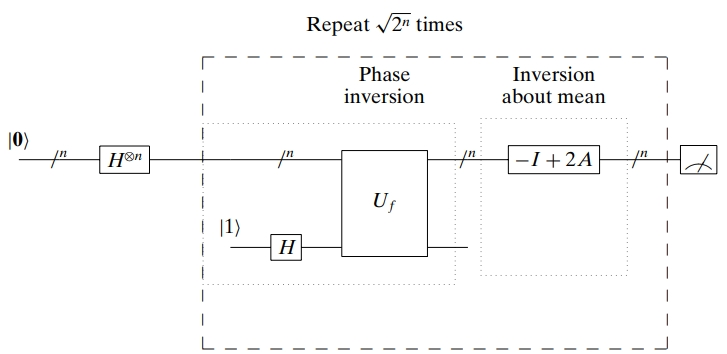
\includegraphics[width=0.7\textwidth]{grovercircuit.jpeg}}
\caption{مدار گراور}
\label{fig:grovercircuit}
\end{figure}
\cite{cambridgebook}
\section{الگوریتم شور}
در سال 1994، پیتر شور
\LTRfootnote{Peter Shor}
با الهام از الگوریتم سایمون
\LTRfootnote{Simon's algorithm}
یک الگوریتم فاکتورگیری کوانتومی با پیچیدگی زمانی چندجمله ای خلق کرد. از سال 1970، محققان به دنبال الگوریتم‌های فاکتورگیری سریع‌تر هستند. پیچیدگی زمانی یک فاکتور مهم در سیستم‌های رمزنگاری است.
\cite{singhbook}
\\
بیشتر امنیت شبکه اینترنت بر مبنای پیچیدگی فاکتورگیری اعداد صحیح توسط کامپیوتر کلاسیک است. الگوریتم شور، به دلیل اهمیت و حساسیت زیاد باعث شد به حوزه محاسبات کوانتومی توجه بیشتری شود.
\cite{cambridgebook}
\\
بهترین الگوریتم فاکتورگیری دارای پیچیدگی زمانی
\begin{equation}
O(e^{cn^{1/3}\log^{2/3}n})
\end{equation}
($n = log_{2}N$ و $N$ عددی است که میخواهیم فاکتورگیری کنیم)
است. این درحالی است که پیچیدگی زمانی الگوریتم شور، 
\begin{equation}
O(n^{2}\log n \log \log n)
\end{equation}
است. که نسبت به $n$ چندجمله‌ای است.
\cite{singhbook}
\\
الگوریتم شور بر اساس یک حقیقت خلق شده است: مسئله فاکتورگیری را به مسئله یافتن تناوب یک تابع تبدیل کرد. 
\cite{cambridgebook}
شور برای پیدا کردن تناوب یک تابع از تبدیل فوریر کوانتومی
\LTRfootnote{quantum Frourier transformation}
بهره‌گیری میکند. همچنین، از توازی کوانتومی
\LTRfootnote{quantum parallelism}
برای ایجاد برهم‌نهی از تمام جواب‌های تناوب تابع استفاده میکند. در برخی از قدم‌های این الگوریتم، از محاسبات کلاسیک هم استفاده میشود.
\cite{singhbook}